\documentclass[
10pt, % Main document font size
a4paper, % Paper type, use 'letterpaper' for US Letter paper
oneside, % One page layout (no page indentation)
%twoside, % Two page layout (page indentation for binding and different headers)
headinclude,footinclude, % Extra spacing for the header and footer
BCOR5mm, % Binding correction
]{scrartcl}
\usepackage{amsmath,amssymb,amsfonts}
\usepackage{latexsym}
\usepackage{graphicx}
\usepackage{verbatim}
\usepackage{booktabs}
\usepackage[usenames,dvipsnames,svgnames,table]{xcolor}

\usepackage[framed,numbered,autolinebreaks,useliterate,final]{mcode}
\usepackage{listings}


\usepackage{multirow}

\usepackage{sectsty}
\sectionfont{\color{NavyBlue}\selectfont}
\subsectionfont{\color{SkyBlue}\itshape\selectfont}

%%%%%%%%%%%%%%%%%%%%%%%%%%%%%%%%%%%%%%%%%
% Arsclassica Article
% Structure Specification File
%
% This file has been downloaded from:
% http://www.LaTeXTemplates.com
%
% Original author:
% Lorenzo Pantieri (http://www.lorenzopantieri.net) with extensive modifications by:
% Vel (vel@latextemplates.com)
%
% License:
% CC BY-NC-SA 3.0 (http://creativecommons.org/licenses/by-nc-sa/3.0/)
%
%%%%%%%%%%%%%%%%%%%%%%%%%%%%%%%%%%%%%%%%%

%----------------------------------------------------------------------------------------
%	REQUIRED PACKAGES
%----------------------------------------------------------------------------------------

\usepackage[
nochapters, % Turn off chapters since this is an article
beramono, % Use the Bera Mono font for monospaced text (\texttt)
eulermath,% Use the Euler font for mathematics
pdfspacing, % Makes use of pdftex�� letter spacing capabilities via the microtype package
dottedtoc % Dotted lines leading to the page numbers in the table of contents
]{classicthesis} % The layout is based on the Classic Thesis style

\usepackage{arsclassica} % Modifies the Classic Thesis package

\usepackage[T1]{fontenc} % Use 8-bit encoding that has 256 glyphs

\usepackage[utf8]{inputenc} % Required for including letters with accents

\usepackage{graphicx} % Required for including images
\graphicspath{{Figures/}} % Set the default folder for images

\usepackage{enumitem} % Required for manipulating the whitespace between and within lists

\usepackage{lipsum} % Used for inserting dummy 'Lorem ipsum' text into the template

\usepackage{subfig} % Required for creating figures with multiple parts (subfigures)

\usepackage{amsmath,amssymb,amsthm} % For including math equations, theorems, symbols, etc

\usepackage{varioref} % More descriptive referencing

%----------------------------------------------------------------------------------------
%	THEOREM STYLES
%---------------------------------------------------------------------------------------

\theoremstyle{definition} % Define theorem styles here based on the definition style (used for definitions and examples)
\newtheorem{definition}{Definition}

\theoremstyle{plain} % Define theorem styles here based on the plain style (used for theorems, lemmas, propositions)
\newtheorem{theorem}{Theorem}

\theoremstyle{remark} % Define theorem styles here based on the remark style (used for remarks and notes)

%----------------------------------------------------------------------------------------
%	HYPERLINKS
%---------------------------------------------------------------------------------------

\hypersetup{
%draft, % Uncomment to remove all links (useful for printing in black and white)
colorlinks=true, breaklinks=true, bookmarks=true,bookmarksnumbered,
urlcolor=webbrown, linkcolor=RoyalBlue, citecolor=webgreen, % Link colors
pdftitle={}, % PDF title
pdfauthor={\textcopyright}, % PDF Author
pdfsubject={}, % PDF Subject
pdfkeywords={}, % PDF Keywords
pdfcreator={pdfLaTeX}, % PDF Creator
pdfproducer={LaTeX with hyperref and ClassicThesis} % PDF producer
} % Include the structure.tex file which specified the document structure and layout

\hyphenation{Fortran hy-phen-ation} % Specify custom hyphenation points in words with dashes where you would like hyphenation to occur, or alternatively, don't put any dashes in a word to stop hyphenation altogether

%----------------------------------------------------------------------------------------
%	TITLE AND AUTHOR(S)
%----------------------------------------------------------------------------------------

\title{\normalfont\spacedallcaps{Numerical Analysis Project \#1 }} % The article title
\author{}
\date{}
\author{\spacedlowsmallcaps{Xinglu Wang}
\\  Student Number: 3140102282
\\ \vspace{0.5em}College of Information Science \& Electronic Engineering} % The article author(s) - author affiliations need to be specified in the AUTHOR AFFILIATIONS block

\date{} % An optional date to appear under the author(s)

%----------------------------------------------------------------------------------------

\begin{document}

%----------------------------------------------------------------------------------------
%	HEADERS
%----------------------------------------------------------------------------------------

\renewcommand{\sectionmark}[1]{\markright{\spacedlowsmallcaps{#1}}} % The header for all pages (oneside) or for even pages (twoside)
%\renewcommand{\subsectionmark}[1]{\markright{\thesubsection~#1}} % Uncomment when using the twoside option - this modifies the header on odd pages
\lehead{\mbox{\llap{\small\thepage\kern1em\color{halfgray} \vline}\color{halfgray}\hspace{0.5em}\rightmark\hfil}} % The header style

\pagestyle{scrheadings} % Enable the headers specified in this block

%----------------------------------------------------------------------------------------
%	TABLE OF CONTENTS & LISTS OF FIGURES AND TABLES
%----------------------------------------------------------------------------------------

\maketitle % Print the title/author/date block

\setcounter{tocdepth}{2} % Set the depth of the table of contents to show sections and subsections only

\tableofcontents % Print the table of contents

\listoffigures % Print the list of figures

%\listoftables % Print the list of tables

%----------------------------------------------------------------------------------------
%	ABSTRACT
%----------------------------------------------------------------------------------------

\section*{Abstract} % This section will not appear in the table of contents due to the star (\section*)
This project is about inner estimation based on Approximation theory(LSE) and natural Cubic Spline interpolation(NCSAPE).
 \\First, I transform normal distribution into linear form. Then use LSE to get an relatively accurate $\mu$ and $\sigma$ for norm distribution. \\Then, I use NCSAPE to get continuous growth curve for $\mu$ and $\sigma$. In this way, we can know the standard height and weight for any month age child.
 \\Meanwhile I consider a  GUI with appropriate  interface. Design an application, interacting with user.
\begin{figure}[tb]
\centering
\subfloat[boyWeight 2D Viewer.]{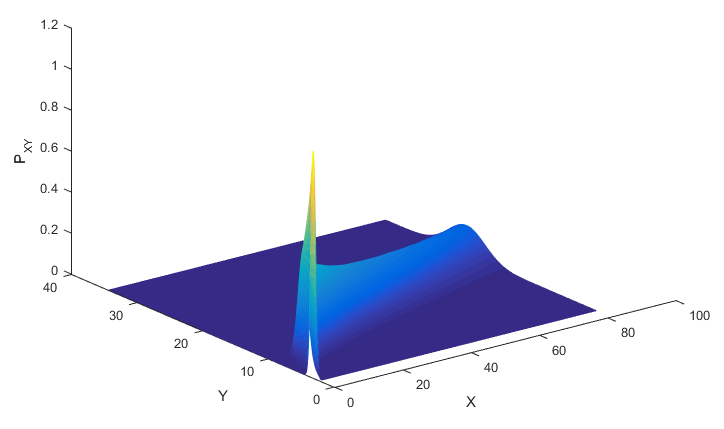
\includegraphics[width=.45\columnwidth]{./fig/overview1.png}} \quad
\subfloat[boyWeight 3D viewer]{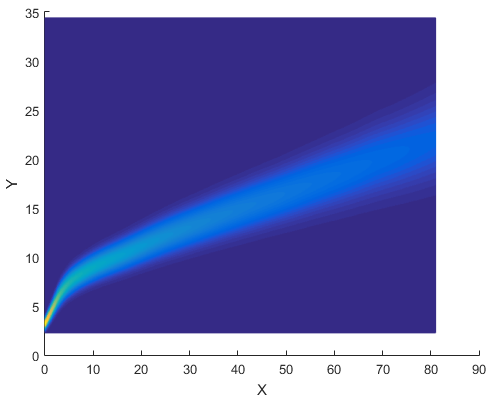
\includegraphics[width=.45\columnwidth]{./fig/overview2.png}} \\
\subfloat[boyHeight 2D viewer]{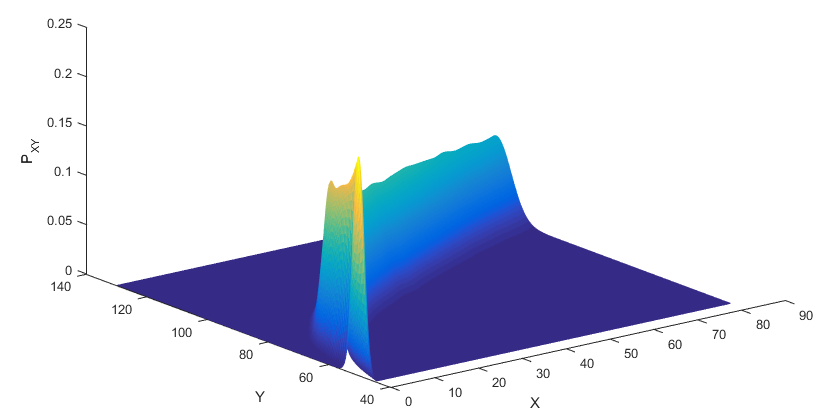
\includegraphics[width=.45\columnwidth]{./fig/overview3.png}} \quad
\subfloat[boyHeight 3D viewer]{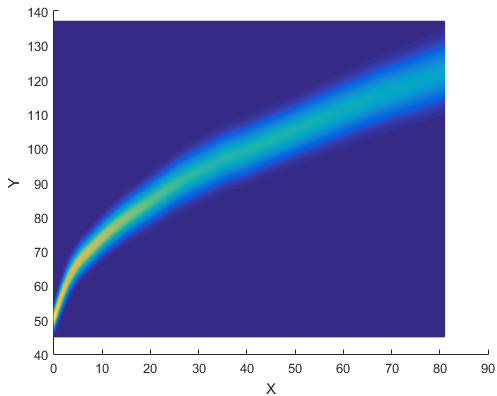
\includegraphics[width=.45\columnwidth]{./fig/overview4.png}}
\caption[A number of pictures for overview.]{A number of pictures for overview.} % The text in the square bracket is the caption for the list of figures while the text in the curly brackets is the figure caption
\label{fig:overview}
\end{figure}


%----------------------------------------------------------------------------------------
%	AUTHOR AFFILIATIONS
%----------------------------------------------------------------------------------------

{\let\thefootnote\relax\footnotetext{* \textit{College of Information Science \& Electronic Engineering, ZheJiang University, China}}}


%----------------------------------------------------------------------------------------

\newpage % Start the article content on the second page, remove this if you have a longer abstract that goes onto the second page

%----------------------------------------------------------------------------------------
%	INTRODUCTION
%----------------------------------------------------------------------------------------

\section{Introduction}

%A statement\footnote{Example of a footnote} requiring citation \cite{Figueredo:2009dg}.
This project is aimed to estimate the standard height and weight of baby and child. Apparently, there many factors that effect the height and weight, so it is difficult to get accurate value. The numerical method can give us deep insight into the complex statistics and provided us with an estimation whose error is acceptable.

%----------------------------------------------------------------------------------------
%	METHODS
%----------------------------------------------------------------------------------------

\section{Interface}
To design an complex system, I first consider its components' interface, which consists of its input and output data flow.
\begin{enumerate}[noitemsep] % [noitemsep] removes whitespace between the items for a compact look
\item A suitable GUI, for user and application.
\item The relationship between each function model.
\end{enumerate}

%------------------------------------------------

\subsection{GUI interface}
First, I design an GUI shown in Figure ~\vref{fig:GUI1}. It is event-drived. Using popupbox to choose boy, girl, weight or height and an convenient calendar to input the birthday of baby.
\\What will be resulted in if user gives an bad INPUT? It is shown in Figure ~\vref{fig:GUI2}.

\begin{figure}[tb]
\centering
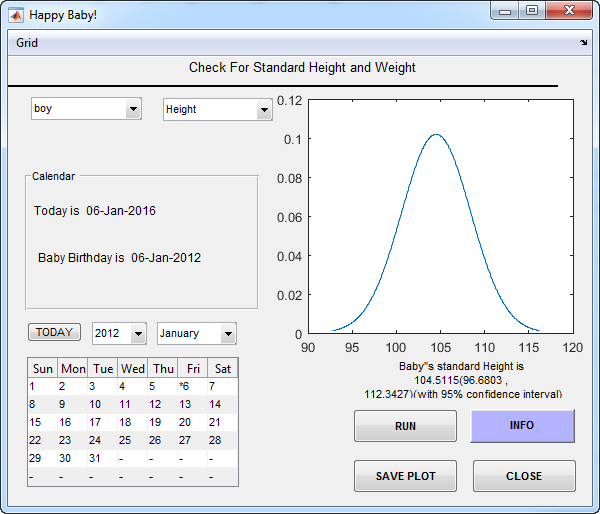
\includegraphics[width=0.5\columnwidth]{../fig/GUI1.png}
\caption[An overview of GUI]{An overview of GUI}
\label{fig:GUI1}
\end{figure}

\begin{figure}[tb]
\centering
\subfloat[So young a baby]{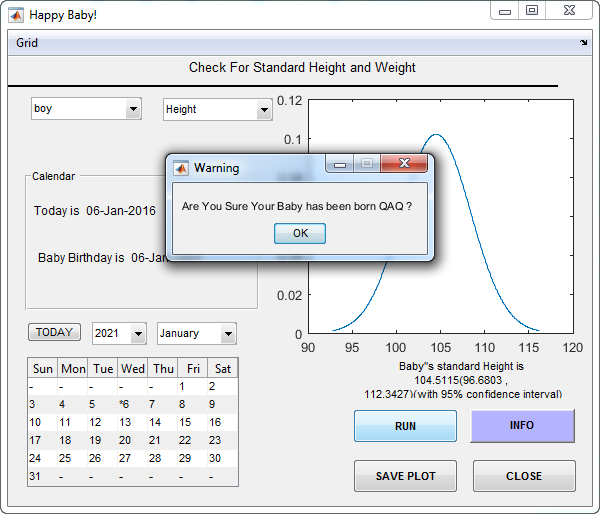
\includegraphics[width=.45\columnwidth]{./fig/GUI2.png}} \quad
\subfloat[So old a baby]{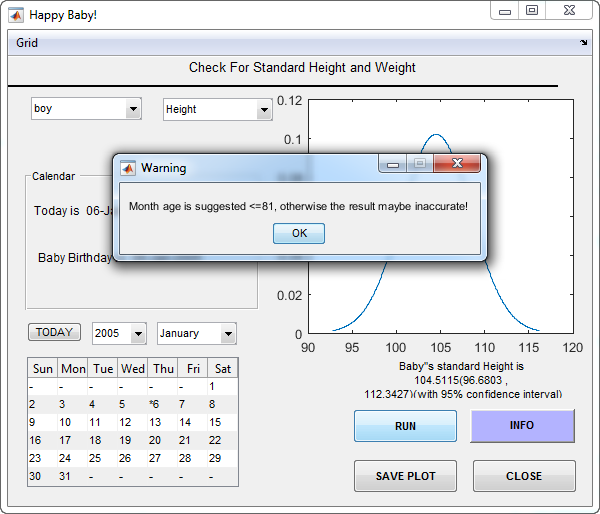
\includegraphics[width=.45\columnwidth]{./fig/GUI3.png}\label{fig:GUI2}}
\caption[A number of pictures.]{A number of pictures with no common theme.}
\end{figure}


\subsection{function interface}
\begin{enumerate}% [noitemsep] removes whitespace between the items for a compact look
\item \mcode{function [year,month,day] = calendarGUI(~,index,action,input)} When input is 'get', it will take time data from calendar on GUI.
\item \mcode {function [mupp,sigpp] = myPre(age,opt)} is the kernel function containing interpolation and approximation algorithm to estimate for any-aged baby.
\end{enumerate}
The relationship between internal function can be complex, there many callback funcion. But basic and main function is calendarGUI(containing \mcode{run_wave_Callback} and \mcode{MainGUI_OpeningFcn}) and myPre(Containing myInterp). The relation can be shown use some tool, but I find it still not very distinct. Reference to Figure ~\vref{fig:rela}
\begin{figure}[tb]
\centering
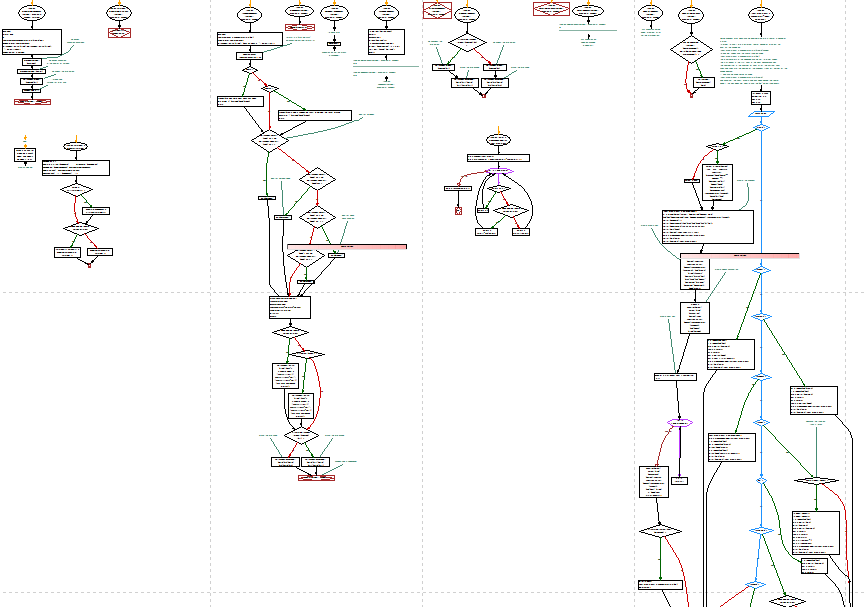
\includegraphics[width=0.5\columnwidth]{./fig/rela.png}
\caption[relationship]{the complex function relation}
\label{fig:rela}
\end{figure}

%------------------------------------------------
\section{Implementation}
\subsection{Overview}
The overview of the complex data is shown on the beginning. Reference to figure  ~\vref{fig:overview}
%\begin{figure}[tb]
%\centering
%\subfloat[boyWeight 2D Viewer.]{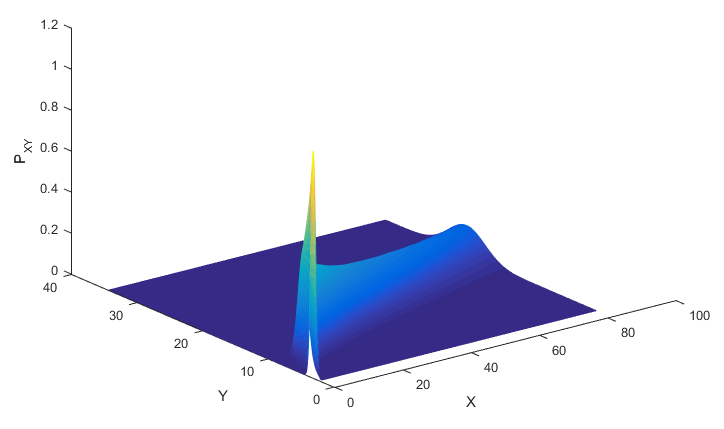
\includegraphics[width=.45\columnwidth]{./fig/overview1.png}} \quad
%\subfloat[boyWeight 3D viewer]{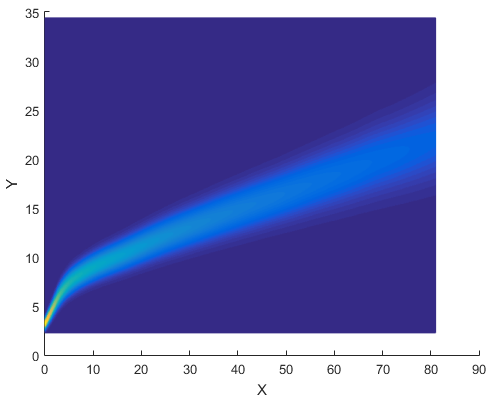
\includegraphics[width=.45\columnwidth]{./fig/overview2.png}} \\
%\subfloat[boyHeight 2D viewer]{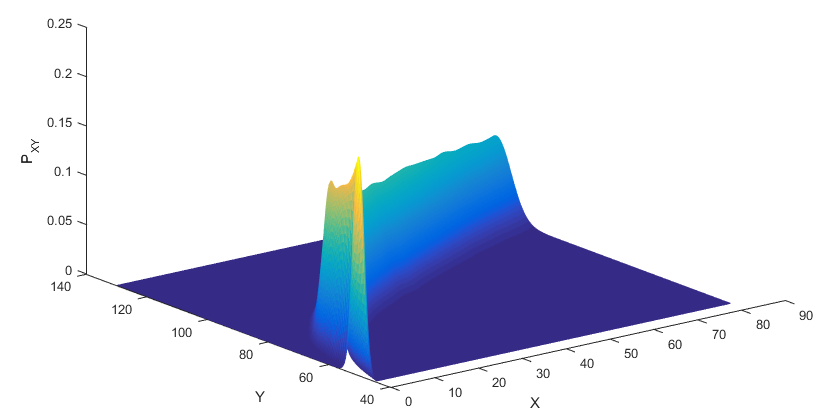
\includegraphics[width=.45\columnwidth]{./fig/overview3.png}} \quad
%\subfloat[boyHeight 3D viewer]{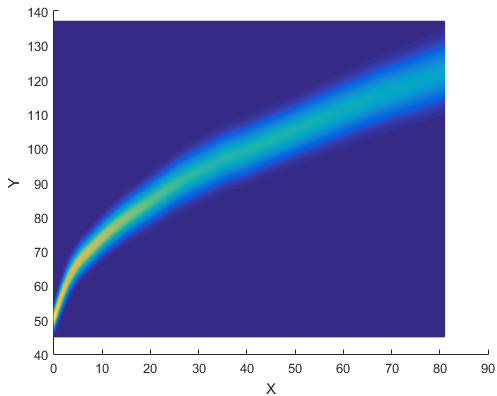
\includegraphics[width=.45\columnwidth]{./fig/overview4.png}}
%\caption[A number of pictures for overview.]{A number of pictures for overview.} % The text in the square bracket is the caption for the list of figures while the text in the curly brackets is the figure caption
%\label{fig:overview}
%\end{figure}
\\First, we can see the data seams very similar to Normal Distribution. We can assume that the sample is mass enough ,therefore the distribution can be viewed as Normal Distribution. So I use the  least square method via some identical transformation to get $\mu$ and $\sigma$ as estimator  for each discrete age's people.
\\Then, we observe from the plot that baby grow more fast than child. Since we do not know the explicit grew function, for accuracy we'd better use interpolation. And I choose cubic spline method.
\\The algorithm flow chart is in  Figure~\vref{fig:scheme}.


\begin{figure}[tb]
\centering
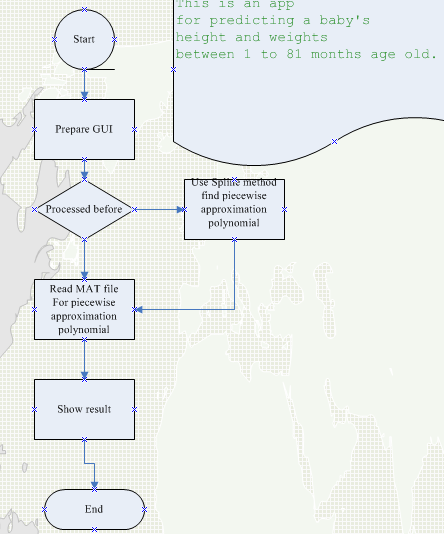
\includegraphics[width=0.5\columnwidth]{./fig/scheme.png}
\caption[flow chart for my algorithm]{flow chart for algorithm} % The text in the square bracket is the caption for the list of figures while the text in the curly brackets is the figure caption
\label{fig:scheme}
\end{figure}
\subsection{Approximation theory(LSE)}
\subsubsection{transform the problem}
First, we can use identical transformation to convert the Normal function into a linear function. We construct $Z = \sqrt {\ln f + \frac{1}{2}\ln 2\pi  + \ln \sigma } $, and submit $f$ with Z
\begin{equation}\label{eq:normpdf}
f(x \; | \; \mu, \sigma) = \frac{1}{\sigma\sqrt{2\pi} } \; e^{ -\frac{(x-\mu)^2}{2\sigma^2} }
\end{equation}
we get
\begin{equation}\label{eq:normlinear}
Z = \frac{x}{{\sqrt {2\sigma } }} - \frac{u}{{\sqrt {2\sigma } }}
\end{equation}
Then, how can we get discrete accurate data form the table shown below?\\


\begin{table}[h]\centering\begin{tabular}{llllllll}
\hline
&-3SD&-2SD&-1SD&mean&+1SD&+2SD&+3SD\\
\hline
{Height}&{\small 44.7}&{\small 46.4}&{\small 48}&{\small 49.7}&{\small 51.4}&{\small 53.2}&{\small 55}\\
\hline
\end{tabular}
\end{table}
We can know the standard normal possibility distribution function (normPDF), then we can get standard possibility dense at $X=\sigma, X=2\sigma $ and so on.
\begin{lstlisting}
mu = 0;
sigma = 1;
x = [-3,-2,-1,0,1,2,3];
standard = normpdf(x,mu,sigma);
\end{lstlisting}
Then we get table shown below:
\begin{table}[h]\centering \begin{tabular}{llllllll}
\hline
&-3SD&-2SD&-1SD&mean&+1SD&+2SD&+3SD\\
\hline
{\small Height}&{\small 44.7}&{\small 46.4}&{\small 48}&{\small 49.7}&{\small 51.4}&{\small 53.2}&{\small 55}\\
\hline
probability dense& 0.0044&0.0540&0.2420&0.3989&0.2420&0.0540&0.0044\\
\hline
\end{tabular}
\end{table}

\subsubsection{Linear Least Square}
\begin{definition}[LSE]
Consider an overdetermined system
$\sum_{j=1}^{n} X_{ij}\beta_j = y_i,\ (i=1, 2, \dots, m)$,
of $m$ linear equations in $n$ unknown coefficients, $\beta_1,\beta_2,...,\beta_n$, with $m > n$.
This can be written in matrix form as
 \[\mathbf {X} \boldsymbol {\beta} = \mathbf {y}\]
where \[
\mathbf {X}=\begin{bmatrix}
X_{11} & X_{12} & \cdots & X_{1n} \\
X_{21} & X_{22} & \cdots & X_{2n} \\
\vdots & \vdots & \ddots & \vdots \\
X_{m1} & X_{m2} & \cdots & X_{mn}
\end{bmatrix} ,
\qquad \boldsymbol \beta = \begin{bmatrix}
\beta_1 \\ \beta_2 \\ \vdots \\ \beta_n \end{bmatrix} ,
\qquad \mathbf y = \begin{bmatrix}
y_1 \\ y_2 \\ \vdots \\ y_m
\end{bmatrix}. \]
 Then, the LSE method is aim at getting an appropriate $\beta$.
\[
\hat{\boldsymbol{\beta}} = \underset{\boldsymbol{\beta}}{\operatorname{arg\,min}}\,S(\boldsymbol{\beta}),\]
where the objective function S is given by
\[
S(\boldsymbol{\beta}) = \sum_{i=1}^{m}\bigl| y_i - \sum_{j=1}^{n} X_{ij}\beta_j\bigr|^2 = \bigl\|\mathbf y - \mathbf X \boldsymbol \beta \bigr\|^2.
\]
\end{definition}

\subsubsection{Fit Result}
To illustrate the fit result, we use boy height at 1 month age old. Reference to Figure ~\vref{fig:norm}. We can see the data is not all pass the fit curve(magnify, and we will see it!), which prove this step is required if we are pursuing for accuracy.
\\But since the original data is from mass sample, the revision of $\sigma$ and $\mu$ is not very remarkable. If we want to implement this application on mobile. We can simply use adjacent data to minus.
\begin{figure}[tb]
\centering
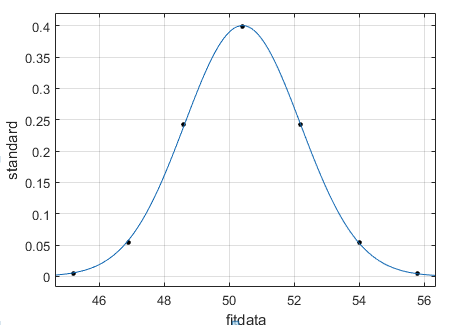
\includegraphics[width=0.8\columnwidth]{../fig/norm.png}
\caption[use LSE to fit normPDF]{use LSE to fit normPDF}
\label{fig:norm}
\end{figure}

\subsection{natural Cubic Spline interpolation(NCSAPE)}
\begin{definition}[CSAPE]
The cubic spline is given by the function values in the nodes and derivative values on the edges of the interpolation interval (either of the first or second derivatives)
\end{definition}
I choose natural CSAPE.
\subsubsection{Why I choose CSAPE?}
The most important reason is that the interpolation error can be made small with 3 degree polynomials for the spline. As a law of natural, children must grow step by step, become taller and stronger gradually. They cannot become very tall suddenly! And CSAPE meets the condition.
\\Cubic Spline interpolation avoids the problem of Runge's phenomenon, in which oscillation can occur between points when interpolating using high degree polynomials. And the Runge's phenomenon is illustrated in ~\vref{fig:runge}
\begin{figure}[tb]
\centering
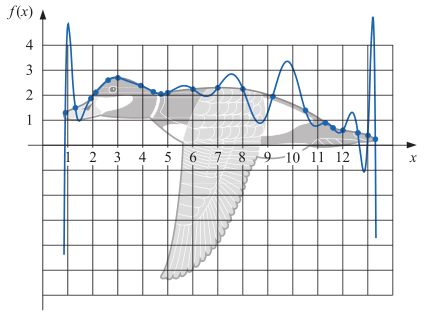
\includegraphics[width=0.5\columnwidth]{./fig/runge.png}
\caption[illustration of Runge's phenomenon]{illustration of Runge's phenomenon}
\label{fig:runge}
\end{figure}
\subsubsection{Why I choose \textbf{natural} CSAPE?}

Let us compare natural CSAPE with clamp CSAPE:
\begin{enumerate}
  \item If the exact values of the first derivative in both boundaries are known, such spline is called clamped spline, or spline with exact boundary conditions. This spline has interpolation error $O(h^4)$.
  \item If the value of the first (or second) derivative is unknown, we can set the so-called natural boundary conditions $S''(A)=0$, $S''(B)=0$. Thus, we get a natural spline. The natural spline has interpolation error $O(h^ 4)$ in the inner nodes. The closer to the boundary nodes the more the error becomes. In the inner nodes the interpolation accuracy is much better.
\end{enumerate}
The reason lies in that we do not know the accurate border message about growth curve, and we won't  inquiry standard data for a unborn baby(too young) and a adult(too old), which means the bound data will in the least be cared for.

\subsubsection{Construct Cubic Spline Interpolate:}As shown below, The construction of the cubic spline is based on the belief that the function value ,derivation and second derivation of the interplant function agree with each other at the nodes.
\begin{center}
  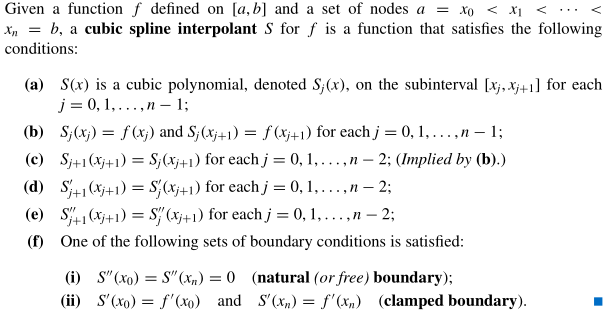
\includegraphics[width=10cm]{./fig/lecture1.png}
\end{center}
Here is cubic spline implement by myself:
\begin{lstlisting}
function pp = myInterp(x,y)
%pp=csape(x',y');
pp = [];
n = length(x);
%% make sure comlumn
[nr, nc] = size(y);
if nr == 1
    y = reshape(y, nc, 1);
    nr = nc;
end
[nr, nc] = size(x);
if nr == 1
    x = reshape(x, nc, 1);
    nr = nc;
end
%%
if size(x) ~= size(y)
    error('x and y are of different size');
end
dx = [0; diff(x); 0];
dxx = dx(1:n) + dx(2:n+1);
% d_xx_j = h_j+h_{j+1}
%%
M = spdiags([[dx(2:n)./dxx(2:n); 0] 2*ones(n,1) [0; dx(2:n)./dxx(1:n-1)]], -1:1, n,n);
dy_l = 0;
dy_r = 0;

b = diff(y) ./ dx(2:n);
c = 6 * diff([dy_l; b; dy_r])./ dxx;

%% For natural spline interpolation
c(1)     = 0;
c(n)     = 0;
M(1,2)   = 0;
M(n,n-1) = 0;
c = M\c;
d = diff(c)./dx(2:n);
b = b  - dx(2:n).* (c(1:n-1)/3 + c(2:n)/6);

%% now compute the values yy
xx=x;
yy = zeros(size(xx));
for i=1:nr-1
    I = find(xx <= x(i+1) & xx >= x(i));
    yy(I) = y(i) + b(i)*(xx(I)-x(i))+c(i)/2*(xx(I)-x(i)).^2 + ...
        d(i)/6*(xx(I)-x(i)).^3;
end
pp=csape(xx,yy);
% c=c(1:end-1);
% y=y(1:end-1);
%% make piecewise poly
%pp=mkpp(x',[d,b,c,y]);
pp = csape(xx,yy);
% Here use csape is only make piecewise ploynomial!
% Becuase my [a,b,c,d] is different from pp-form in matlab. But I want to
% use its plot function. To use its fit-function is just for convenience! 
\end{lstlisting}
And the result for boy height CSAPE is shown below:
\begin{center}
  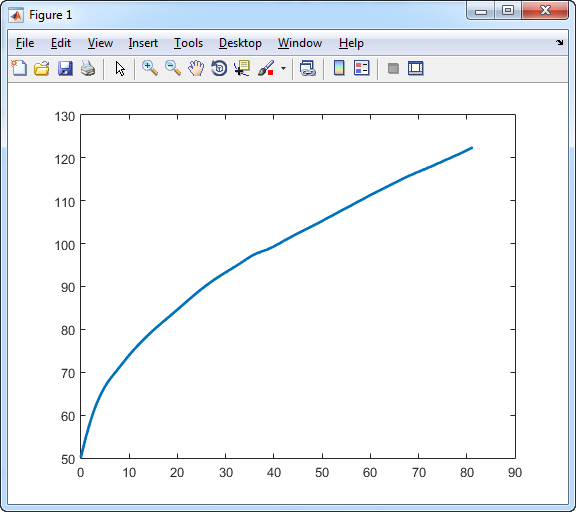
\includegraphics[width=.5\columnwidth]{./fig/CSresult.png}
\end{center}
\subsubsection{Uniqueness of natural CSAPE}
\begin{theorem}
If $f$ is defined at $a = x_0 < x_1 < ... < x_n = b$,then $f$ has a unique natural spline interpolant S; that is, a spline interpolant that satisfies the natural boundary is unique.
\end{theorem}
\begin{proof}
Use the continuity and derivation condition, we can get an linear equation system that specifies our CSAPE.\\
The matrix A is strictly diagonally dominant, that is, in each row the magnitude of the
diagonal entry exceeds the sum of the magnitudes of all the other entries in the row.A linear
system with a matrix of this form have a
unique solution.
\begin{center}
  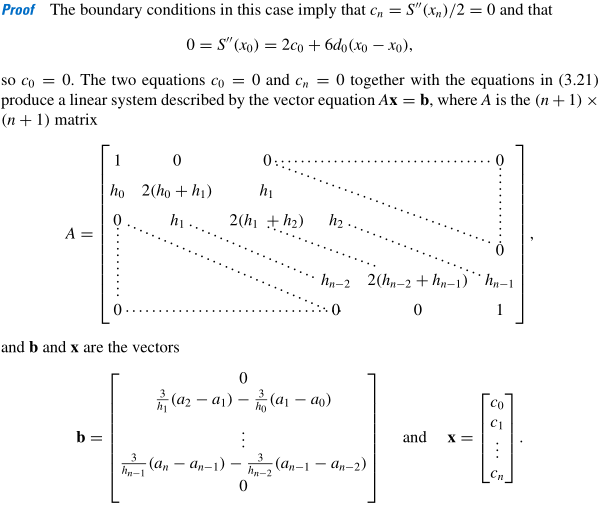
\includegraphics[width=10cm]{./fig/lecture2.png}\\
\end{center}
\end{proof}
\section{Discussion}

\subsection{Complexity analysis}
The total computational complexity is $O(C^2N)$. Reference to the analysis of Matlab ~\vref{fig:complex}
\begin{figure}[tb]
\centering
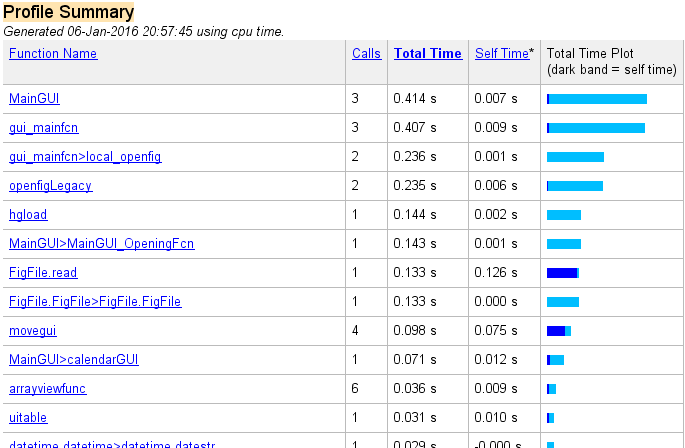
\includegraphics[width=0.5\columnwidth]{./fig/complex.png}
\caption[the complexity]{the complexity}
\label{fig:complex}
\end{figure}
\subsubsection{For LSE}
Refer to normal equation --- $\beta=(X^TX)^{-1}X^Ty$, we can conclude that it costs $O(C^2N)$
\subsubsection{For CSAPE}
We can solve the well-posed linear system with iteration method, so it cost $O(N)$.

\subsection{Improvement(SSAPE)}
As we believe, children grow gradually, which means the curve of growth must be as smooth as possible. So there are more suitable method to approach the curve ---- Smoothing Spline(SSAPE).\\
Understand the notion visual oriented, we can refer to Figure ~\vref{fig:CSAPEVSSSAPE}

\begin{figure}[tb]
\centering
\subfloat[smoothing spline]{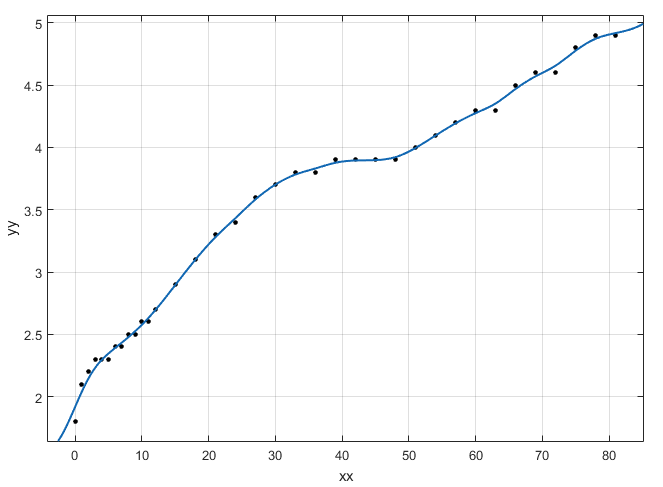
\includegraphics[width=.45\columnwidth]{./fig/smoothRes.png}\label{fig:CSAPEVSSSAPE}} \quad
\subfloat[cubic spline]{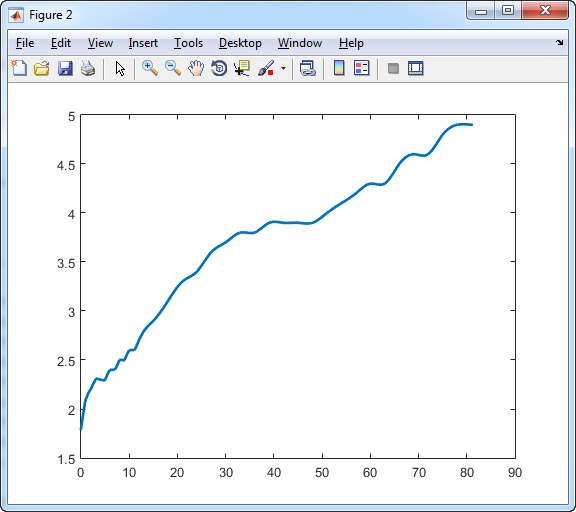
\includegraphics[width=.45\columnwidth]{./fig/notsmooth.png}}
\caption[CSAPE V.S. SSAPE]{CSAPE V.S. SSAPE}
\end{figure}


SSAPE adds an roughness penalty function to the objective function and use the method of optimization to avoid affection of  noisy observations.

\begin{definition}[Smoothing Spline]
Let $(x_{i},Y_{i})$;$x_{1}<x_{2}<\dots <x_{n},i\in \mathbb {Z}$  be a sequence of observations, modeled by the relation $Y_{i}=\mu (x_{i})$. The smoothing spline estimate ${\hat {\mu }}$ of the function $\mu$  is defined to be the minimizer (over the class of twice differentiable functions) of

\begin{equation}
\sum _{i=1}^{n}(Y_{i}-{\hat {\mu }}(x_{i}))^{2}+\lambda \int _{x_{1}}^{x_{n}}{\hat {\mu }}''(x)^{2}\,dx
\label{eq:smooth}
\end{equation}
\end{definition}


And we can use the matlab function to achieve our idea. 
\begin{lstlisting}
function fitresult=SmoothingSpline(X,Y)
%% Using smoothing spline.
ft = fittype( 'smoothingspline' );
opts = fitoptions( 'Method', 'SmoothingSpline' );
opts.SmoothingParam = 0.115222516467702;
[fitresult, ~] = fit( X', Y', ft, opts );
figure;
plot( fitresult, X', Y' );
\end{lstlisting}







\section*{Appendix}
Attach the MainGUI function:
\lstinputlisting{../project/MainGUI.m}
\end{document}
